\section{Design}

In order to filter out noisy data and prepare clean access sequence for training,
we will isolate the sub I/O sequences by dealing with the following challenges.
First, visiting addresses of the sub I/O sequences may not necessarily follow simple pattern, e.g. sequential.
Second, multiple concurrent workloads mix their individual requests in one I/O stream and result in many one-time-access patterns.
To handle the challenges, one simple solution is to let application pass along its identity,
e.g. file id or process id, to the storage system.
However, this is intrusive to the system when we pass kernel level ID information to application level.
More importantly, the number of files or transactions being accessed from one application or I/O channel is big.
In today's multi-core machines, passing all the ids to the one layer becomes infeasible.
As a result, we will develop an unsupervised stream classification algorithm to learn the hidden heuristics from upcoming I/O sequences.

\subsubsection*{Temporal-Aware Sequence Classification}

To classify the I/O sequence,
one key is to identify appropriate features.
Researchers from Google apply k-means classification to perform main memory
footprint analysis, identify the sub I/O sequences and feed them
to individual RNN models~\cite{hashemi2018learning, peled2018towards}.
The classification of CPU to memory accesses is well matched with
the segment classification function of k-means.
First, the CPU time is multiplexed by the applications using the time-sharing technique,
in a given timesegment we can assume there is only one application accessing the memory.
Second, the physical memory addresses shared by the applications are segmented by the operation system.
However, these two assumptions are not applied to external I/O access classification.

We propose a fine-grained \emph{temporal-aware sequence classification} algorithm
to find the sequence relations by using a sliding time window.
We aim to discover the hidden relation being buried in address domain,
and project our trace records to a new multi feature domain
by considering the record correlation hidden in the time series.
The convergence algorithm is being developed to implement a projection protocol
taking both address and time series info of data into consideration.

According to our observation in experiments, with the multi-threaded I/O trace,
the naive application of those methods have merely slight better prediction accuracy than random guess,
and even no better than predicting based on simple statistics.
Nonetheless, they achieve an outstanding performance on single-threaded trace,
which has low space locality and is a difficult problem for traditional methods.

Due to the specific internal data structures of various kinds of applications,
there exists repeated access patterns in the trace.
However, modern operation systems generally execute a mixture of a large number of I/O workloads concurrently.
These concurrent workloads interweave their I/O sequences stochastically.
This is substantially different to the DRAM workloads.
Because, the DRAM workloads mainly share the DRAM bandwidth based on the time sharing mechanism in a multi-core CPU.
However, the external I/O workloads share the resources through the hardware interrupts.
In the consolidated I/O sequence, the amount of the noise requests substantially exceed that of the original requests.
Therefore, it is important and difficult to first discover access sequence of each individual workload from an entangled trace.

We hypothesize the correlation of I/O requests is implicit in I/O traces.
Specifically, two or more requests are supposed to be strongly correlated if their have been accessed together in short time intervals repeatedly.
According to this observation, we split the consolidated I/O sequence into multiple sub I/O sequences based on the address correlation.
Thus, the requests within a sub sequence have a significant higher correlation than those across subsets.
On the contrary, the interlaced trace is segregated based on the division of the address been requested.
And each trace split is likely to be belonging to one or a few correlated transactions and with reduced noise.

\begin{figure}[h]
\centering
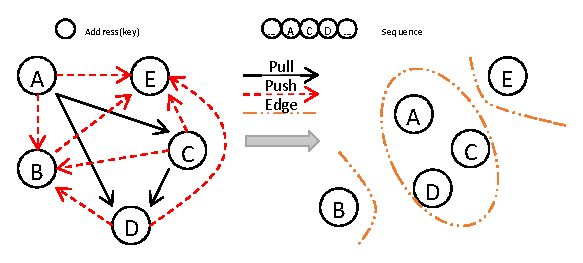
\includegraphics[width=0.9\linewidth]{fig/sequence_grouping.eps}
\caption{Temporal-aware Sequence Classification.}
\label{fig:sequence_grouping}
\end{figure}

We propose \emph{Temporal-Aware Sequence Classification (TAC)},
an unsupervised learning-based approach to solve the problem.
The idea is to split the address sequence
and disentangle the multi-thread effects in I/O request trace
according to their temporal correlation.
TAC share part of the idea from both graph processing and clustering algorithms.
Comparing to clustering RNN~\cite{hashemi2018learning},
TAC makes no assumption about the spatial locality of addresses.
Instead, it scrutinizes the low-level I/O trace based on correlated addresses
information from their time stamps.
Given specific complexity and feasibility,
we will develop two distinct protocols to implement TAC.

\emph{Probabilistic-based Approach:}
To deal with $M$ addresses and $N$ potential groups, we maintain a $M\times N$ matrix
as the probability table.
Each entry in the table represents the probability that specific address is
affiliated with the target group.
The objective is to maximize the probability that a cluster of addresses being
correlated could be assigned to a same group.

We observe that strong correlated cells are likely to be accessed
by one thread in succession, thus tend to appear in short intervals
in the entangled trace.
Therefore, we give a big weight to strengthen the virtual link
between each pair of addresses which emerge in a fixed-length time window
and update the probability table according to those links.
Specifically, the probability that a cell is affiliated with a group is determined by the probabilities that the cells appeared in previous time window are affiliated with that group.
Given an increasing number of accesses to a certain cell,
its correlated cells will obtain a higher chance to be accessed together
and thus make a larger impact than others.
To quantify the principle, we develop an updating formula shown in Equation~\ref{eq:probabilitisticbasedequation} for the cells in the probability table:

\begin{equation}
\label{eq:probabilitisticbasedequation}
P_{dst} = (1 - \lambda) \cdot P_{dst} + \lambda \cdot mean(P_{src})
\end{equation}

in which $dst$ denotes the address which probability to be updated,
while $src$ denotes a list of cells linked to $dst$ with in the time window, and $\lambda$ is an updating factor.

When the table converges to a stable state, each address is assigned to a certain group based on its maximum likelihood.
At the end, according to corresponding group assignment of cells,
the trace is split into multiple independent single-threaded sequences
and then fed into RNN to make predictions.
Although statistical-based approach captures the correlations as well,
it might suffer from the following issues:
First, there lacks a fairness distribution policy.
The approach tends to assign all the cells to one or a few.
Second, upon processing a large number of groups,
probabilities affiliated with each group become small.
Due to the large amount of noise in trace,
the model tends to overact a tiny change in the table,
and unnecessarily switch the assignment.
Third, the complexities of both time and space have a linear relation
to the number of groups, which tell it is unrealistic to implement
in real-world environment.

\emph{Physical-based Approach:}
To address the issues of the statistical-based approach, as shown in Figure~\ref{fig:sequence_grouping},
we propose physical-based approach which procedure is similar but essentially different.
Instead of binding the addresses with a probability matrix,
As shown in Figure~\ref{fig:sequence_grouping}, we adopt a physical-based approach which
maps the addresses to points in a $N$-dimensional linear space.
Upon the arrival of the requests, the points of correlated cells apply attractive force to each other while the uncorrelated ones apply repulsive force.
As the points moving in the space, they will gradually form clusters while those clusters will be separated by repulsion.
In this process, the repulsive force serves as regularization and makes the points more equally distributed.
For example, if address A, C and D appeared together in the sequence sliding window,
the algorithm will pull them closer in the N-dimensional space,
so that the classification algorithm can categorizes them into one class.
On the convergence of the movement, clustering algorithms are adopted to assign the points into groups.
With the combination of the physical movement and clustering, this approach obtains a better division as well as being robust to noise.

\begin{equation}
\label{eq:physicalbasedequation}
feature_{dst} = (1 - \lambda) \cdot feature_{dst} + \lambda \cdot mean(feature_{src})
\end{equation}

Moreover, in some cases, highly correlated addresses share a close accessing frequency.
An additional term is introduced to reflex this consideration by applying extra movement based on their access frequency.
And a frequency factor is involved to lever the weight of this term, which is adjustable for specific file systems and applications.
The equation for this term is in Equation~\ref{eq:frequencyterm}:

\begin{equation}
\label{eq:frequencyterm}
feature = (1 - \epsilon) \cdot feature + \epsilon \cdot frequency
\end{equation}
in which $\epsilon$ represents the frequency factor.
% And the complete procedure of TAC is presented in Algorithm~\ref{tacphysical}.

In real-world scenario, the number of concurrent threads is varying over time.
The physical-based approach maps the addresses based on their correlation rather than setting hard boundaries on division,
which makes it possess the potential to solve this issue.
% We leave this exploration to future work.

\iffalse
\begin{algorithm}
\caption{The procedure of TAC algorithm}
\label{tacphysical}
\begin{flushleft}
\textbf{Input:} $trace$, $ng$(number of groups), $interval$, $criterion$, $\lambda$(updating factor), $\epsilon$(frequency factor)
\linebreak
\textbf{Output:} $mp$(mapping table)
\end{flushleft}
\begin{algorithmic}[1]
  \State $na \gets$ \#addresses appeared in trace
  \State $freq \gets$ normalized frequency of addresses appearance
  \State $table \gets$ random matrix of $na \times ng$
  \State $table \gets \textbf{Standardize}(table)$
  \State $step \gets criterion + 1$
  \While{$step > criterion$}
    \State $target \gets$ \textbf{Target}($trace,na,ng$)
    \State $step \gets \textbf{mean}(target-table)$
    \State $table \gets (1-\lambda) \cdot table + \lambda \cdot target$ \Comment apply attractive force
    \State $table \gets (1-\epsilon) \cdot table + \epsilon \cdot freq$ \Comment extra movement regularized by frequency
    \State $table \gets \textbf{Standardize}(table)$ \Comment{expansion as repulsion}
  \EndWhile
  \State $mp \gets \textbf{Clustering}(table)$
  \State \textbf{return} $mp$
\end{algorithmic}
\hspace{0.6cm}- - - - - - - - - - - - - - - - - - - - - - - - - - - - - - - -
\begin{algorithmic}[1]
  \Function{Standardize}{$table$}
    \State $\mu \gets$ mean $w.r.t.$ rows of $table$
    \State $\sigma \gets$ deviation $w.r.t.$ rows of $table$
    \State $table \gets (table - \mu) / \sigma$
    \State \textbf{return} $table$
  \EndFunction
\end{algorithmic}
\hspace{0.6cm}- - - - - - - - - - - - - - - - - - - - - - - - - - - - - - - -
\begin{algorithmic}[1]
  \Function{Target}{$trace,na,ng$}
    \State $target \gets$ zero matrix of $na \times ng$
    \For{$dst$ in $trace$}
      \State $src \gets$ addresses appeared within
      \State \hspace{1.05cm}$interval$ before $dst$ in $trace$
      \State $target(dst) \gets target(dst)+mean(table(src))$
    \EndFor
    \State \textbf{return} $target$
  \EndFunction
\end{algorithmic}
\end{algorithm}
\fi

\iffalse
\begin{figure}[h]
\centering
\includegraphics[width=0.9\linewidth]{fig/multi_scale_grouping.eps}
\caption{Illustration of Multi-scale Workload Identification.}
\label{fig:multi_scale_grouping}
\end{figure}

\subsubsection*{Step 2: Multi-scale Workload Classification}

It is common to physically isolate the data from different applications both
for the performance and security purpose~\cite{huang2017flashblox}.
This ispire us to do multi-scale classification.
To achieve this, we need to submit the application's information together with the I/O requests to the low level disks,
which needs a large investment of changes in the storage subsystem.
It is more challenge when virtualization technique are deployed.
For example, system managers would use different filesystem configurations
for different applications.
However, if the managed system runs in a virtualized environment,
it would be more challenge to config properly.
Another solution is to estimate the necessary information
based on the learned I/O patterns,
so that we can develop an automatic performance tuning technique.
This lays in the fact that different application
will generate significantly different I/O pattern.
We can use a sequence classification technique to identify the workloads,
and then enable different workload-aware optimization methods.
Not only the application I/O, we may also identify the system workloads,
such as distinguish the filesystem from the I/O pattern.
To solve this, we propose to do multi-scale workload classification as shown in Figure~\ref{fig:multi_scale_grouping}.
In the first layer, we do cross-grained classification to distinguish different types of workloads.
As a result, substantially different workloads can be isolated.
Then in the second layer, we can further apply our temporal-aware classification
to study fine-grained request relationships.
\fi
